\documentclass[12pt]{article}

\usepackage[margin=1.0in]{geometry}
\usepackage{color}
\usepackage{times}
\usepackage{graphics}

\pagestyle{empty}
\setlength{\parindent}{0in}
\setlength{\parskip}{2ex}
\renewcommand{\baselinestretch}{1.0}

\begin{document}

STAT 604: \hfill {Mu-Fen Hsieh}\\
Intro.\ to Statistical Computing \hfill {Sep. 14, 2006}

\begin{center}
\Large HW 3\\
\end{center}

In this report, I will show both theoretically and empirically that Marilyn Vos Savant is correct. That is, the strategy to switch
 the door is to the advantage of the contestant.
 
First, to use Bayes rule, we assume that the doors are named $A$, $B$ and $C$, and that the contestant chooses door $A$ at the beginning. 
Then we define some events:\\
\begin{center}
$PA$: The prize is behind the door $A$.\\
$PB$: The prize is behind the door $B$.\\
$PC$: The prize is behind the door $C$.\\
$OA$: The door $A$ is opened by the host.\\
$OB$: The door $B$ is opened by the host.\\
$OC$: The door $C$ is opened by the host.\\
$CA$: The door $A$ is later chosen by the contestant.\\
$CB$: The door $B$ is later chosen by the contestant.\\
$CC$: The door $C$ is later chosen by the contestant.
\end{center}

The probabilities of event $PA$, $PB$, $PC$ are the same. That is, $P(PA)=1/3$, $P(PB)=1/3$ and $P(PC)=1/3$. The probability that the host will 
open the door $B$ is calculated.
\begin{eqnarray}P(OB) & = & P(PA) \times P(OB|PA) + P(PA) \times P(OB|PA) + P(PA) \times P(OB|PA) \nonumber \\
& = & 1/3 \times 1/2 + 1/3 \times 0 + 1/3 \times 1 = 1/2\end{eqnarray}
There are three possibilities. Since the contestant chose door $A$, if the prize were behind $A$, the game host can choose either to open 
door $B$ or door $C$. Thus the probability to open door $B$ is 1/2. If the prize were behind $B$, the host will never open door $B$. If the 
prize were behind door $C$, the host will certainly open door $B$.

Under the same assumption that door $A$ is picked at the beginning, now we calculate the winning probability when the contestant sticks 
to door $A$ (Fig. 1a) and when the contestant switches to door $C$ (Fig. 1b), given that the host opened door $B$. 
\begin{eqnarray}P(CA|OB) & = & P(CA) \times P(OB|CA) / P(OB) = 1/3 \times 1/2 / 1/2 = 1/3\\
                P(CC|OB) & = & P(CC) \times P(OB|CC) / P(OB) = 1/3 \times 1 / 1/2 = 2/3\end{eqnarray}
We can see that to stick to the original choice will give a winning probability of $1/3$, which is half the winning probability of taking the switch.

The empirical experiment is done secondly. A different way of analyzing the problem is used. We assume that the prize is randomly assigned 
to one of the door with probability $1/3$ and that the contestant chooses one of the door with probability $1/3$ as well. Then two possibilities 
are discussed. One is that the door chosen at the beginning is the one with a prize (Fig. 1b). The other is that the door chosen is not 
with a prize (Fig. 1a). In the former case (Fig. 1b), if the contestant switches the door, they surely will lose. If not, they will win. 
In the latter case (Fig. 1a), the situation is inversed. If the contestant does not take the switch, they will lose. However, after the game 
host opened a door, the contestant will win if they take the switch.

\begin{figure}[h]
\centering
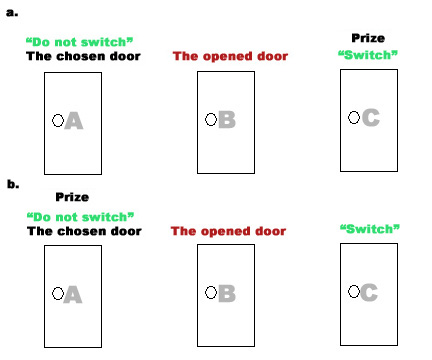
\includegraphics{MontyHall.jpg}
\caption{The two cases which might occur in the game.}
\end{figure}

My experiment is implemented based on the two possibilities mentioned. In the first step, the door of prize and the contestant's beginning 
choice is randomly assigned by $1$, $2$ or $3$, which is corresponding to the three doors. We assume that there are two contestants who adopt 
different strategies but make identical choices at the beginning. Then, whether the contestants win or lose is determined by checking if 
the door of prize was picked at the beginning. The number of trials is 125000.

In the statistics of the results, similar probabilities to the theoretical results were obtained.
\begin{eqnarray}P(\textit{winning under strategy ``switch''}) & = & 0.664192\textit{, with a confidence interval } \nonumber \\
& & [0.6615738, 0.6668102] \textit{ and the estimated } \nonumber \\
& & \textit{ variance } 0.472274. \nonumber \\
P(\textit{winning under strategy ``do not switch''}) & = & 0.335808\textit{, with a confidence interval } \nonumber \\
& & [0.3331898, 0.3384262] \textit{ and the estimated } \nonumber \\
& &\textit{ variance } 0.472274. \nonumber \end{eqnarray}
The mean of probability of winning under strategy ``switch'' is close to $2/3$, and the mean of probability of winning under strategy ``do not 
switch'' is close to $1/3$. 

My conclusion is that to switch the door gives the contestant a higher probability to win.

\end{document}
